%%%%%%%%%%%%%%%%%%%%%%%%%%%%%%%%%%%%%%%%%%%%%%%%%%%%%%%%%%%%%%%%%%%%%%%%%%%%%%%%%%%%%%%%%%
\section{Discussion}

%%%%%%%%%%%%%%%%%%%%%%%%%%%%%%%%%%%%%%%%%%%%%
\subsection{Manual feature selection}

% sklearn random forest  

\begin{table}[H]
    \centering
    \caption{Ranking of feature importance from best to worst with respect to
    impurity decrease for three different reconstruction methods on the full
    dataset obtained with sci-kit learn.}  
    \label{tab:feature_importance}  

    \begin{tabular}{|c|c|c|c|}
        \hline
        Rank & Feature index & Feature name & Impurity decrease \\     
        \hline
        0       & 2           & histogram min  & 0.102915  \\
        1      & 12            & glcm entropy  & 0.088981  \\
        2      & 11           & glcm contrast  & 0.083777  \\
        3       & 4           & histogram std  & 0.081181  \\
        4      & 13        & glcm homogeneity  & 0.080463  \\
        5       & 5      & shape area\_density  & 0.073690  \\
        6       & 3          & histogram peak  & 0.069483  \\
        7       & 0           & histogram max  & 0.064857  \\
        8      & 14      & glcm joint\_maximum  & 0.061548  \\
        9       & 9    & shape volume\_density  & 0.055089  \\
        10      & 8            & shape volume  & 0.051088  \\
        11      & 7           & shape surface  & 0.048897  \\
        12     & 10            & glcm cluster  & 0.048494  \\
        13      & 1          & histogram mean  & 0.047758  \\
        14      & 6  & shape convex\_hull\_area  & 0.041778  \\
        \hline
         
    \end{tabular} 
\end{table}


% Identify features with poor class separation

% Identify highly correlated features  
% * plot correlation matrix  

\begin{figure}[H]
    \centering
    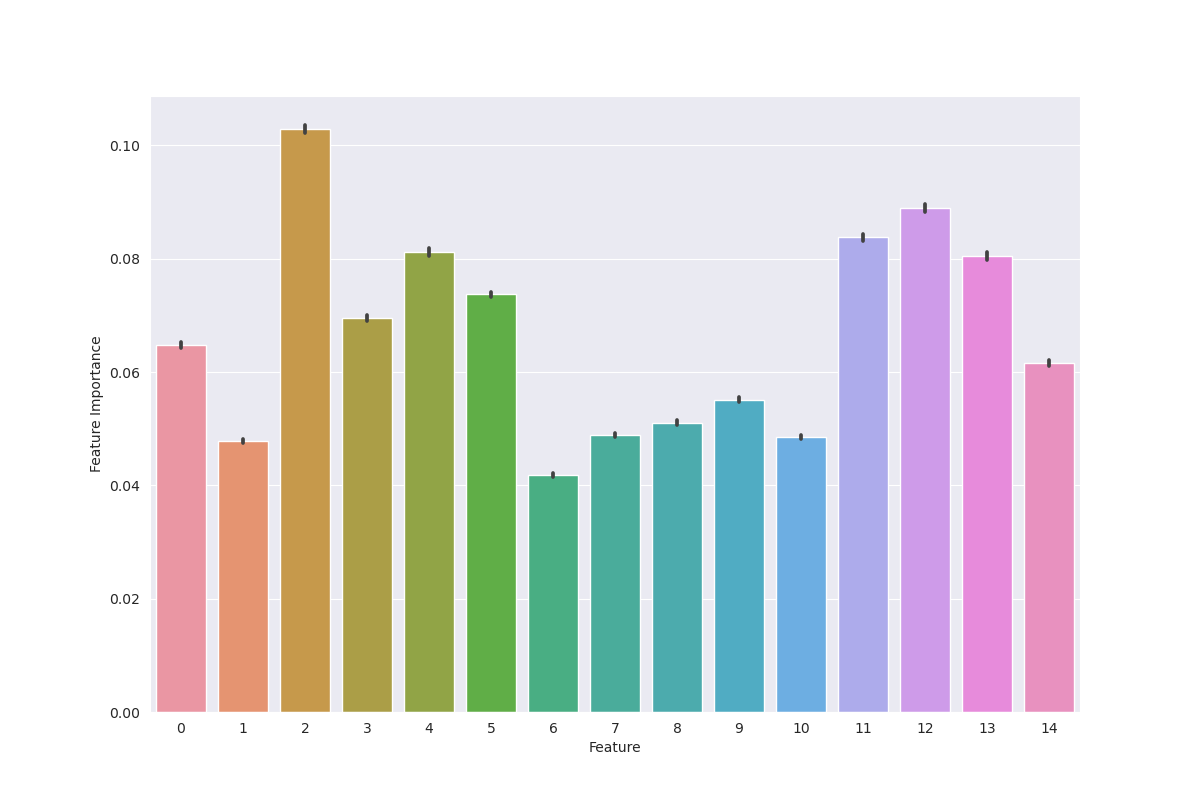
\includegraphics[width=0.8\textwidth]{Figures/feature_importance_sklearn_3s.png}
    \caption{Mean of the feautre\_importacnes\_ (purity decrease) for each decision tree. The
    error bar shows the 95\% confidence interval. The x-axis represent feature
    number as defined in table \ref{tab:feature_names}.  }  
    \label{fig:feature_importance} 
\end{figure}


\begin{figure}[H]
    \centering
    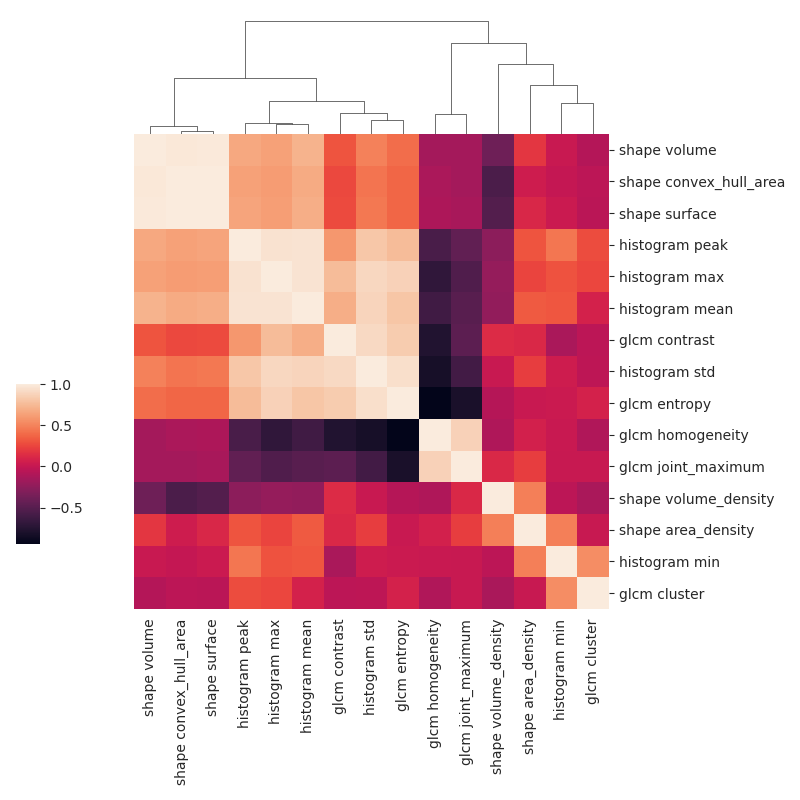
\includegraphics[width=1\textwidth]{Figures/feature_correlation.png}
    \caption{Pearson Correlation between each feature calculated on the full
    dataset. }  
\end{figure}





%%%%%%%%%%%%%%%%%%%%%%%%%%%%%%%%%%%%%%%%%%%%%
\subsection{Compare Manual VS Automatic feature reduction}
\begin{itemize}
    \item Is the Automatic selection method as expected, compared with visual
        inspection, manual feature reduction.   
\end{itemize}




%%%%%%%%%%%%%%%%%%%%%%%%%%%%%%%%%%%%%%%%%%%%
\subsection{SVM}

\subsubsection{Classification of class 1 vs class 4}

\begin{figure}[H]
\centering
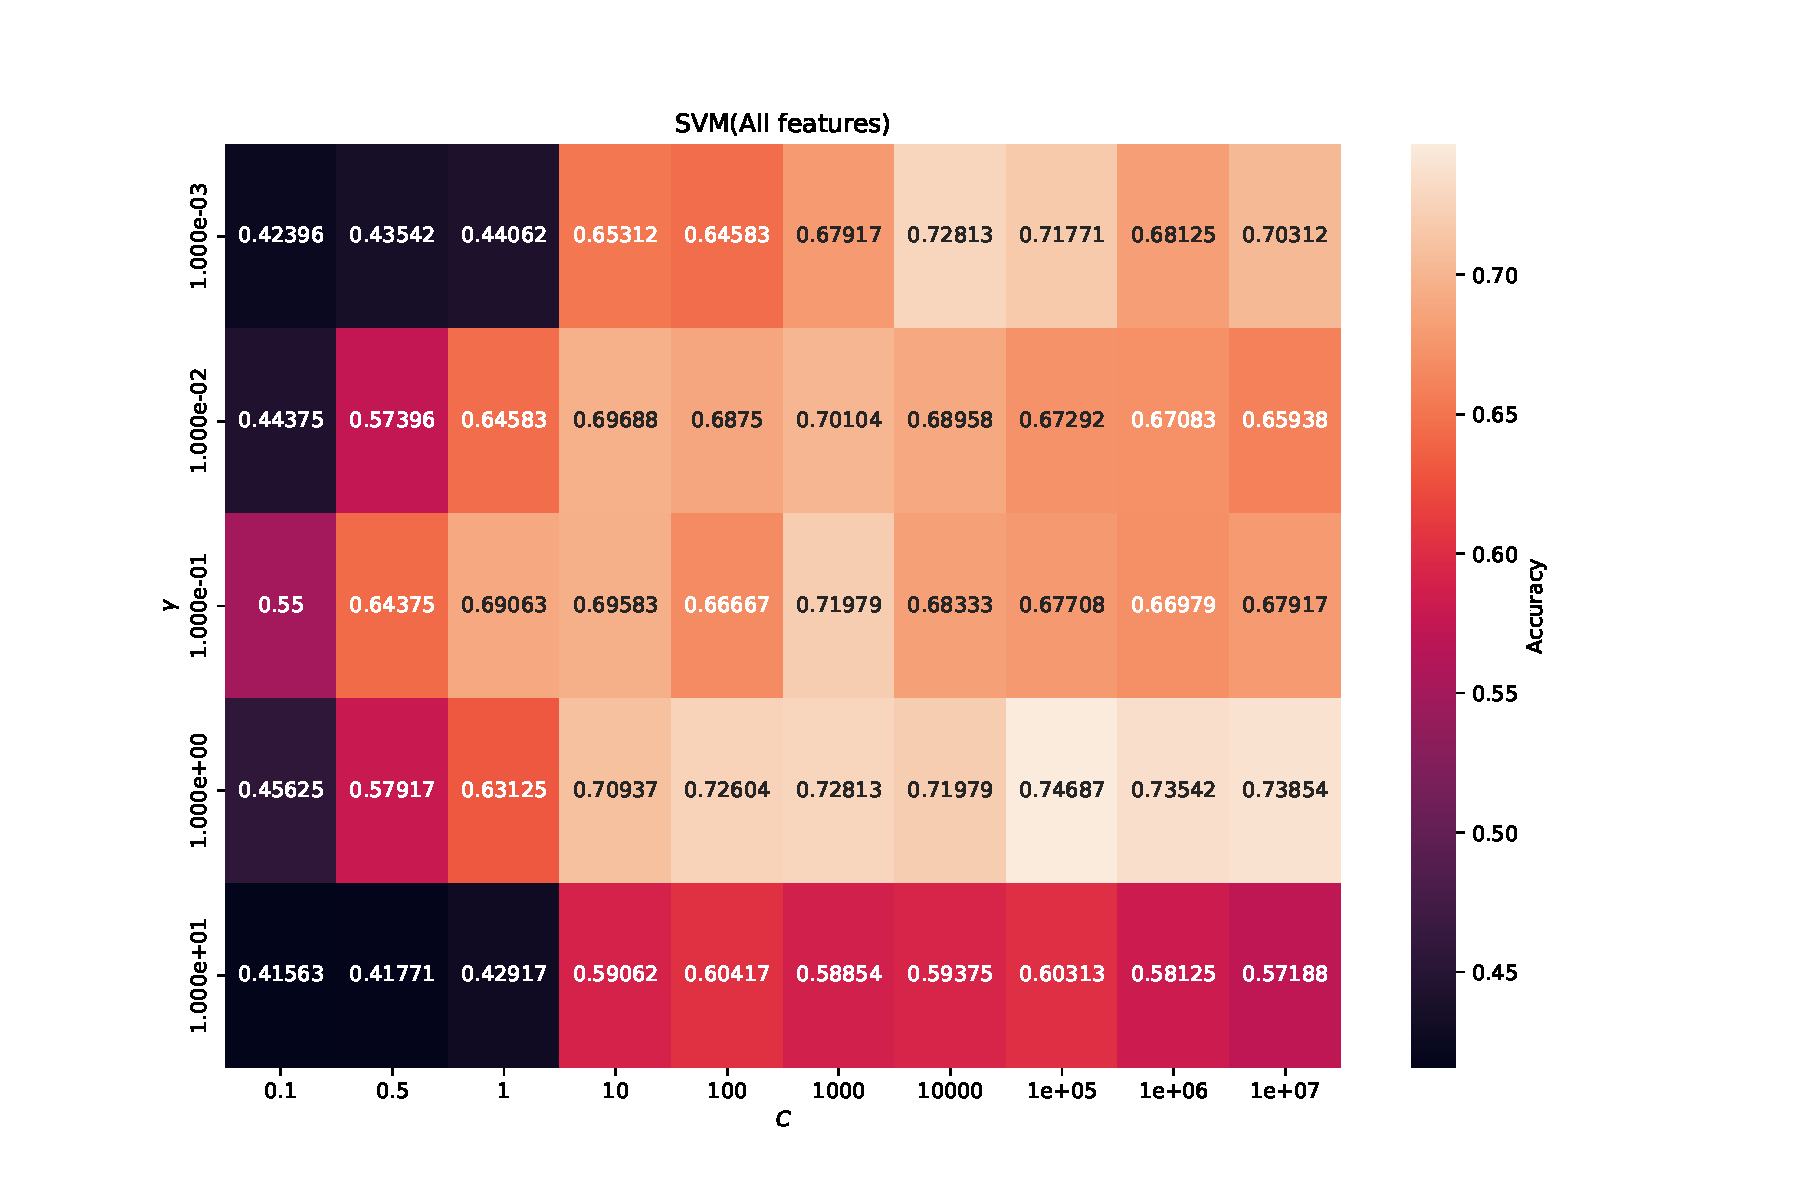
\includegraphics[width=1\textwidth]{Figures/accuracy(C,gamma)0}
\caption{Heatmap of the accuracy obtained with different slack constants $C$ and 
GRBF kernel factors $\gamma $ in the SVM model training with all the features. The SVM accuracies are the average of $30$ cross-validation 
cycles training and predicting test data of relative size $0.25$.}
\label{fig:Figures-accuracy-C-gamma-0}
\end{figure}

\begin{figure}[H]
\centering
\makebox[\textwidth][c]{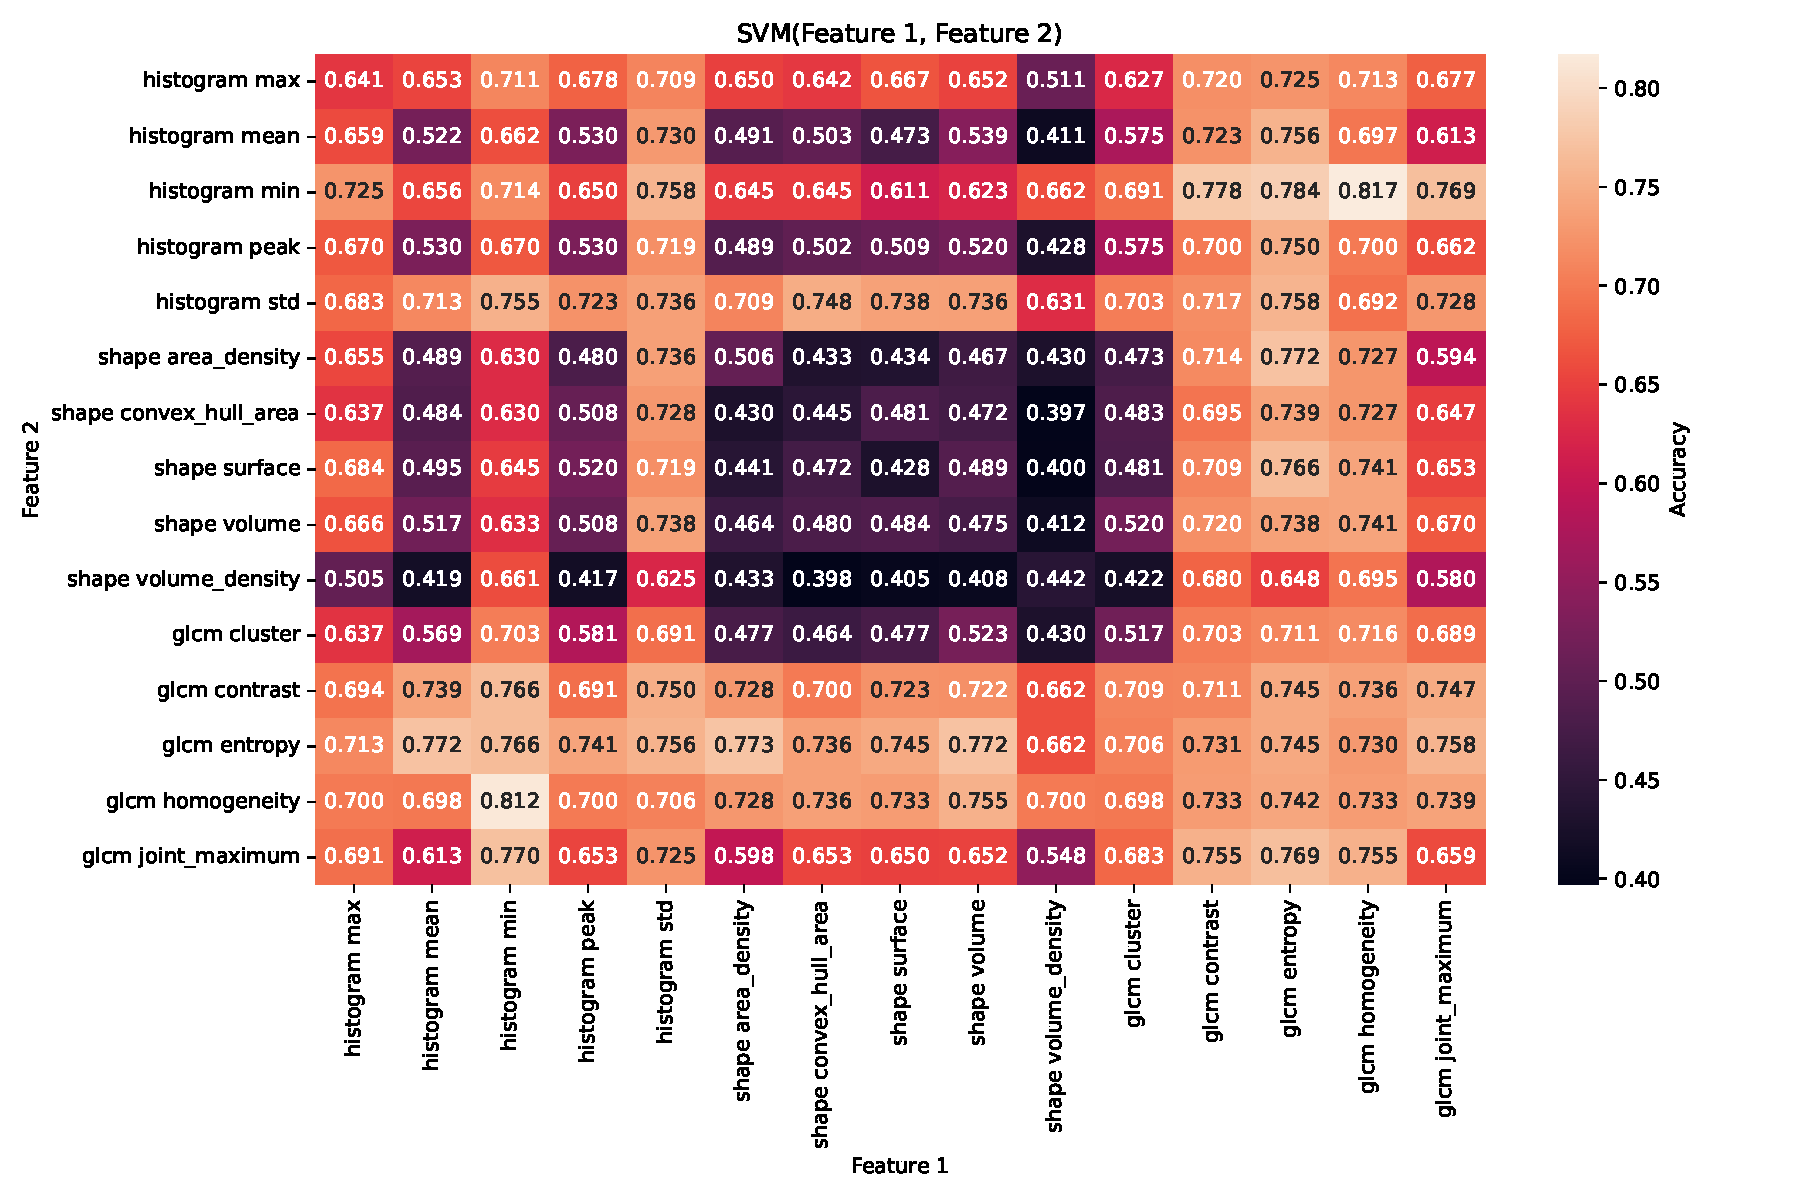
\includegraphics[width=1.2\textwidth]{Figures/feature_pairs0}}
\caption{Heatmap of the accuracy obtained by the SVM model training on different feature pairs. The SVM accuracies are the average 
of $20$ cross-validation cycles training and predicting test data of relative size $0.25$.
The slack constant and GRBF kernel factor are set to $C=10^5$  $\gamma=1 $ respectively. }
\label{fig:Figures-feature_pairs0}
\end{figure}

\begin{figure}[H]
\centering
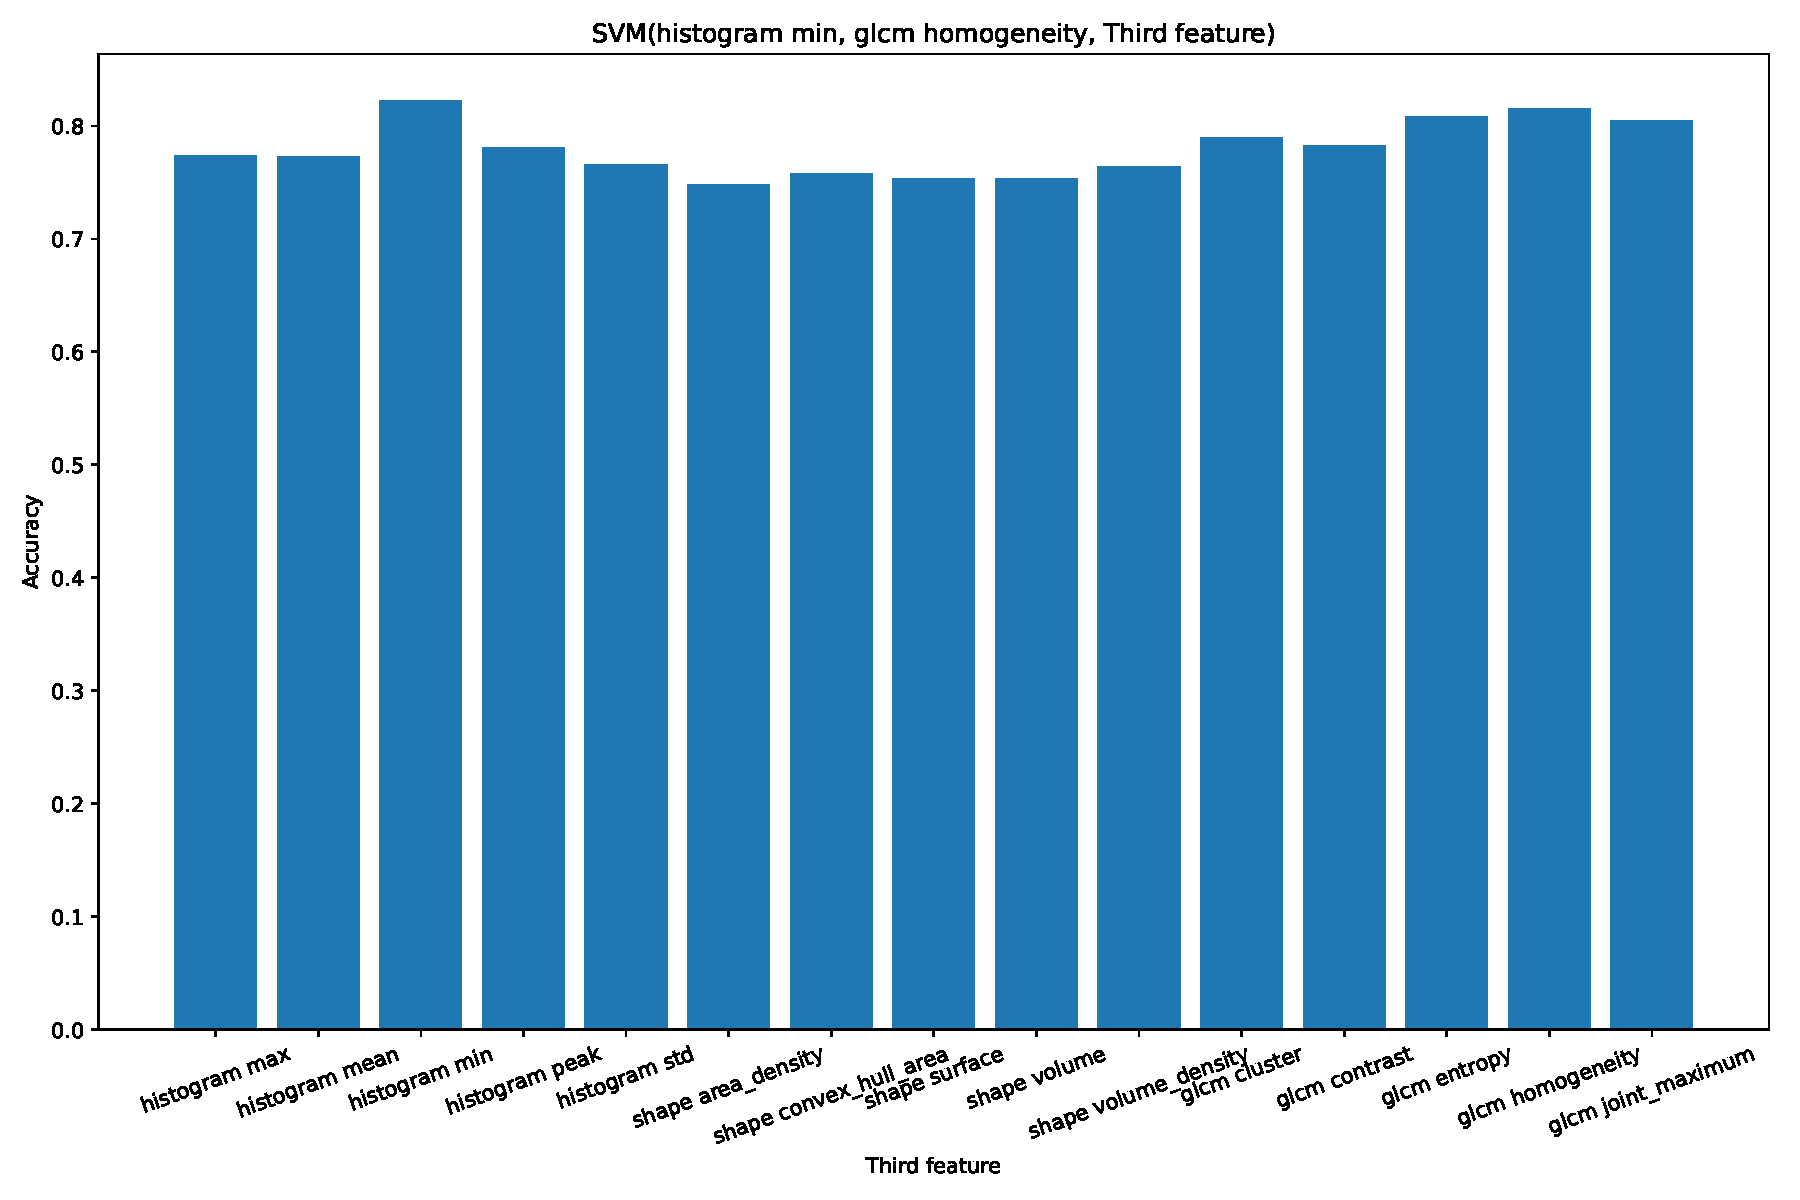
\includegraphics[width=1\textwidth]{Figures/third_feature0}
\caption{Bar plot of the accuracy obtained adding a third feature in the data used 
by the SVM model. The accuracies are the average 
of $50$ cross-validation cycles training and predicting test data of relative size $0.25$.
The slack constant and GRBF kernel factor are set to $C=10^5$  $\gamma=1 $ respectively. }
\label{fig:Figures-third_feature0}
\end{figure}

\subsubsection{Classification of class 0 vs class 4}

\begin{figure}[H]
\centering
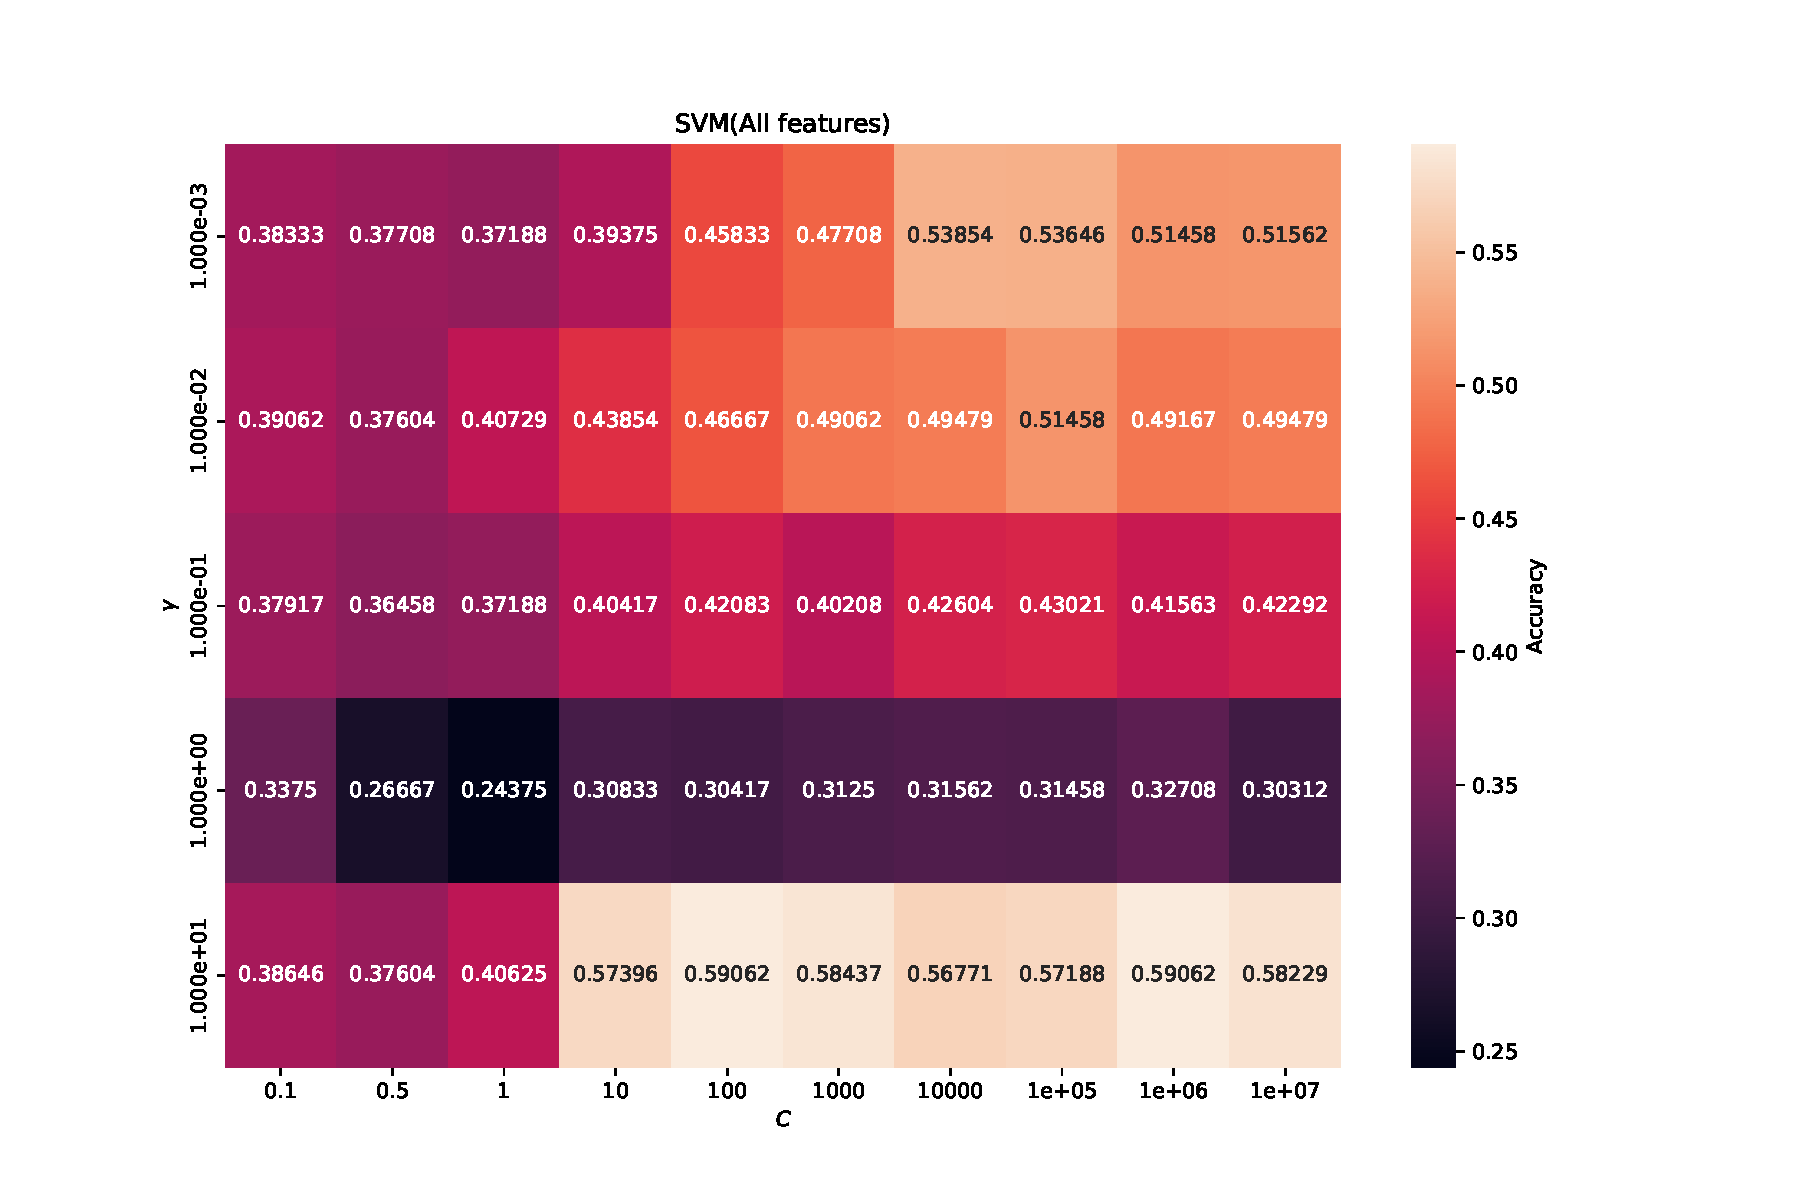
\includegraphics[width=1\textwidth]{Figures/accuracy(C,gamma)1}
\caption{Heatmap of the accuracy obtained with different slack constants $C$ and 
GRBF kernel factors $\gamma $ in the SVM model training with all the features. The SVM accuracies are the average of $30$ cross-validation 
cycles training and predicting test data of relative size $0.25$.}
\label{fig:Figures-accuracy-C-gamma-1}
\end{figure}

\begin{figure}[H]
\centering
\makebox[\textwidth][c]{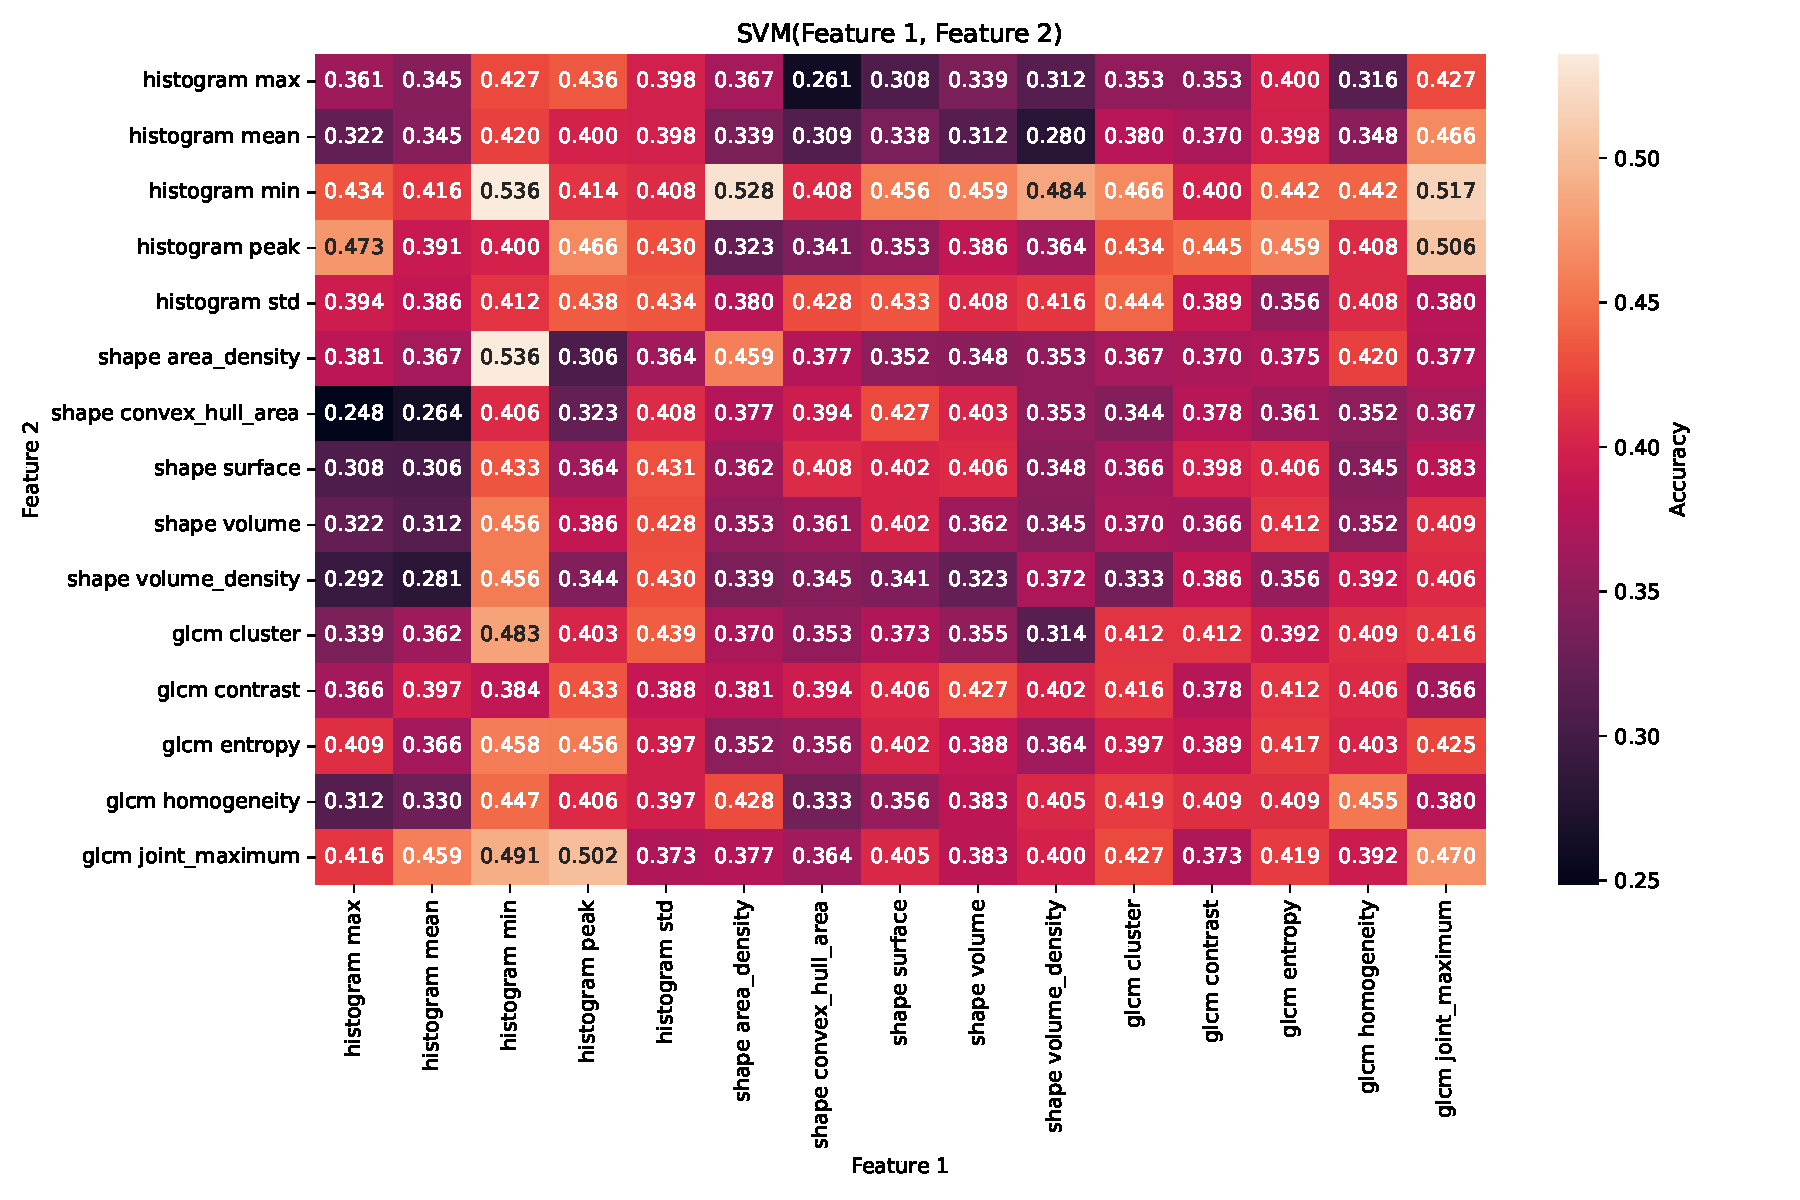
\includegraphics[width=1.2\textwidth]{Figures/feature_pairs1}}
\caption{Heatmap of the accuracy obtained by the SVM model training on different feature pairs. The SVM accuracies are the average 
of $20$ cross-validation cycles training and predicting test data of relative size $0.25$.
The slack constant and GRBF kernel factor are set to $C=100$  $\gamma=10 $ respectively. }
\label{fig:Figures-feature_pairs1}
\end{figure}

\begin{figure}[H]
\centering
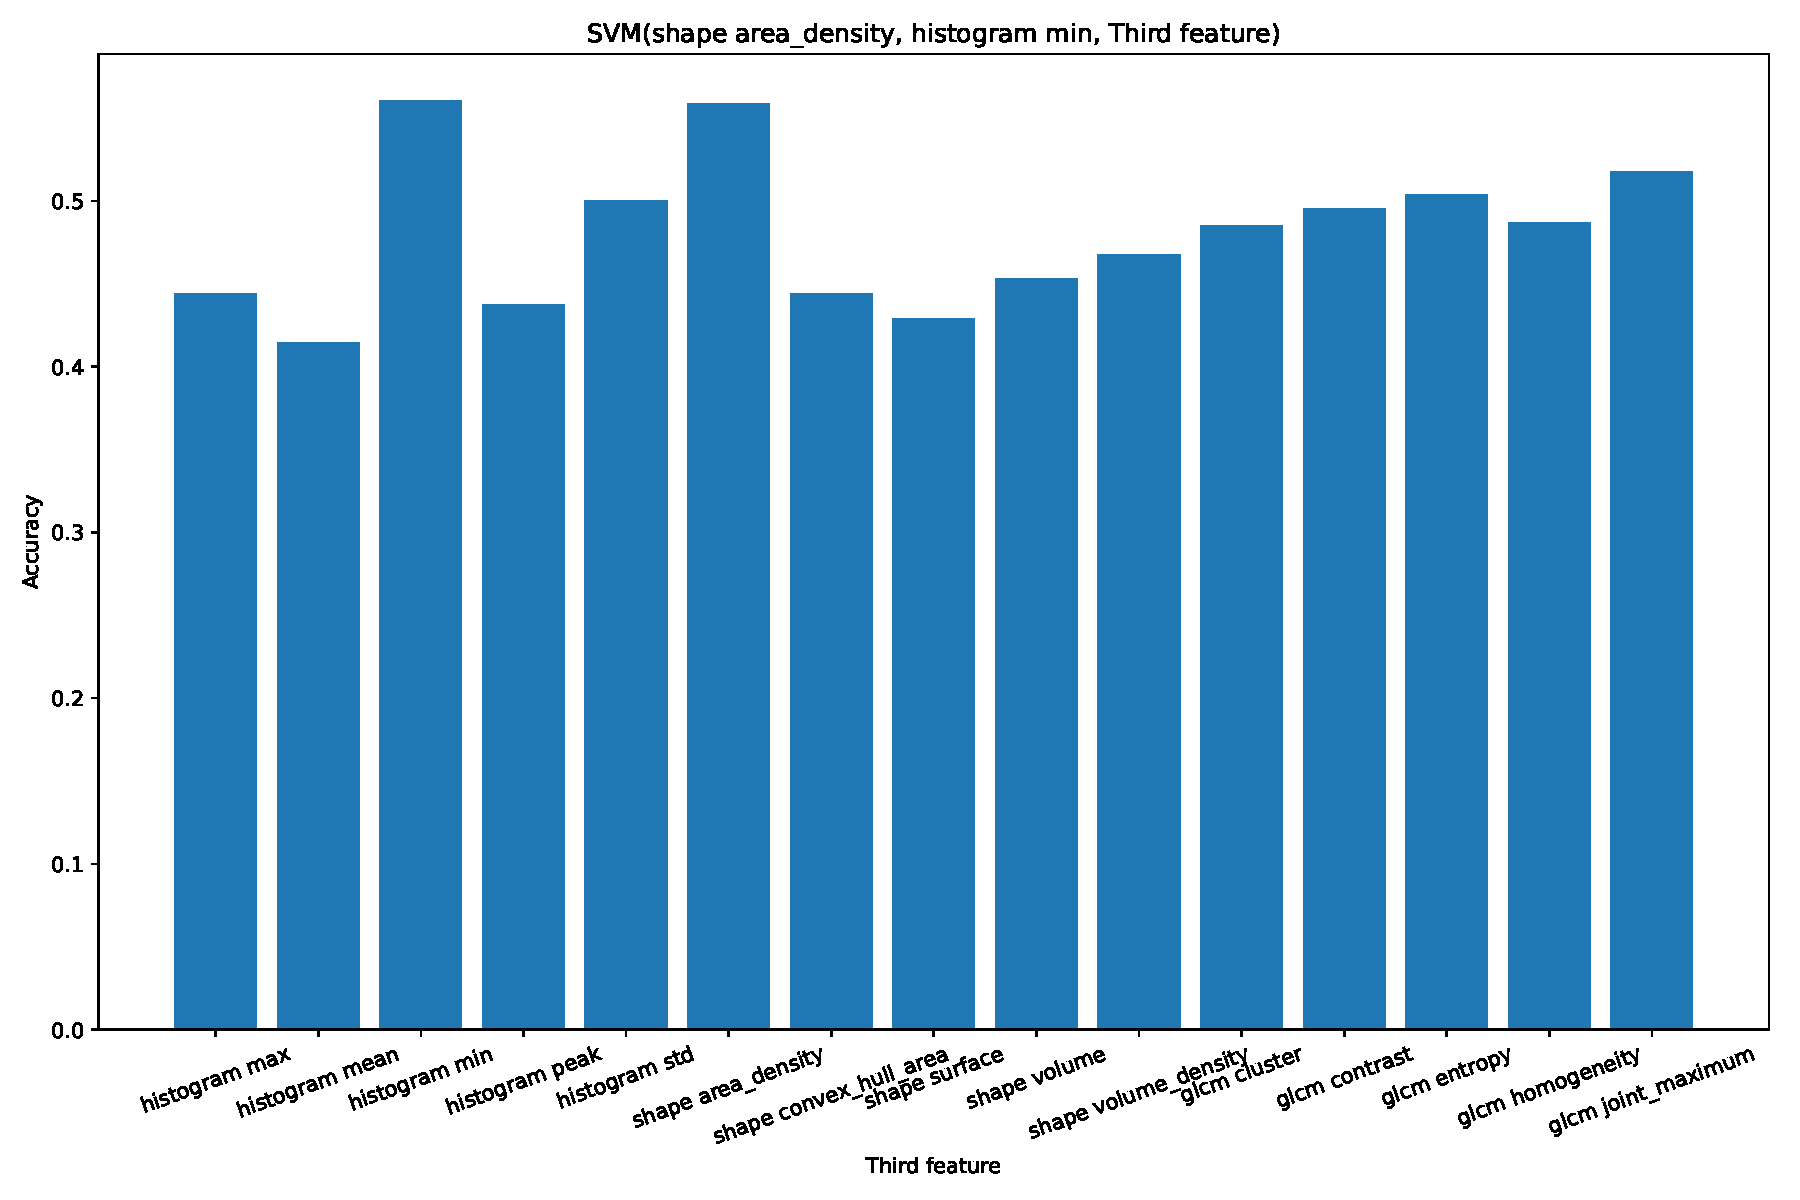
\includegraphics[width=1\textwidth]{Figures/third_feature1}
\caption{Bar plot of the accuracy obtained adding a third feature in the data used 
by the SVM model. The accuracies are the average 
of $50$ cross-validation cycles training and predicting test data of relative size $0.25$.
The slack constant and GRBF kernel factor are set to $C=100$  $\gamma=10 $ respectively. }
\label{fig:Figures-third_feature1}
\end{figure}


\subsubsection{Classification of class 0 vs class 1}

\begin{figure}[H]
\centering
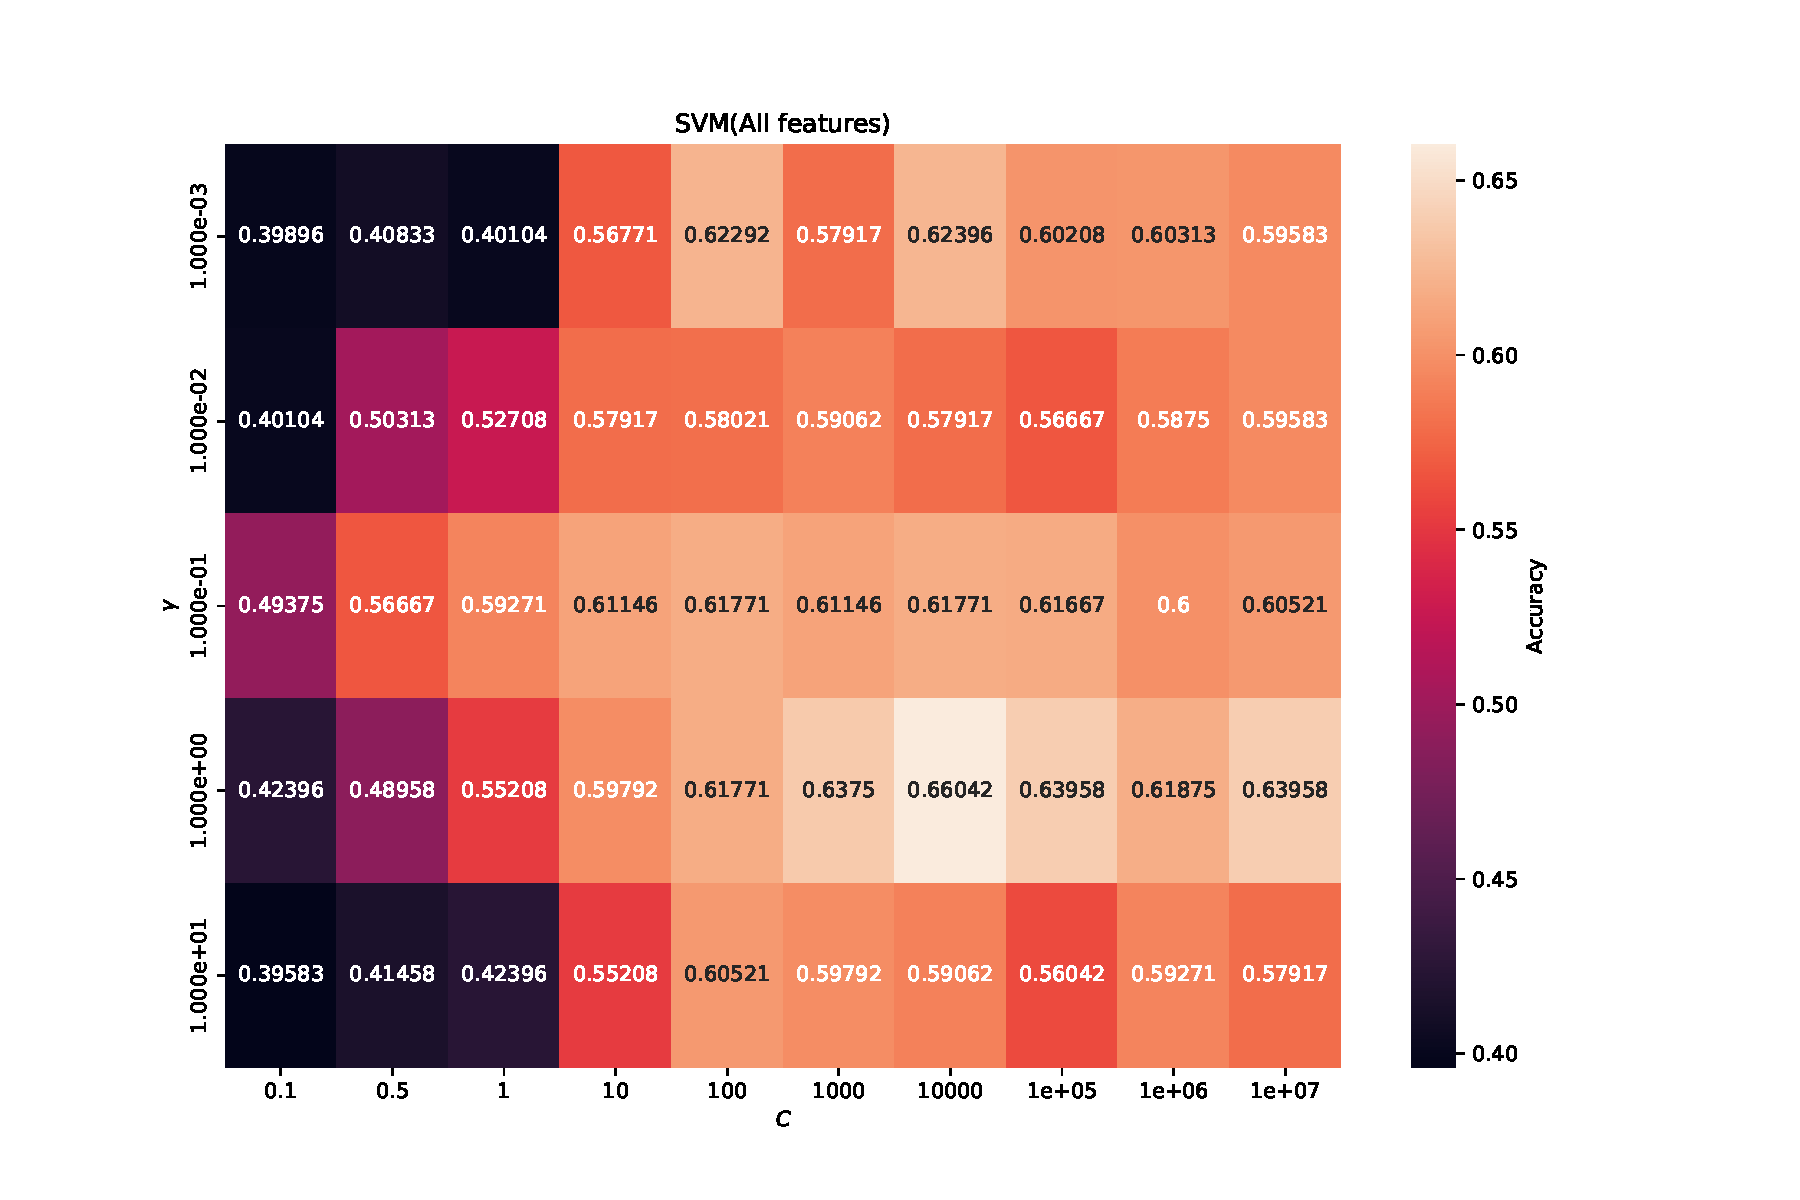
\includegraphics[width=1\textwidth]{Figures/accuracy(C,gamma)4}
\caption{Heatmap of the accuracy obtained with different slack constants $C$ and 
GRBF kernel factors $\gamma $ in the SVM model training with all the features. The SVM accuracies are the average of $30$ cross-validation 
cycles training and predicting test data of relative size $0.25$.}
\label{fig:Figures-accuracy-C-gamma-4}
\end{figure}

\begin{figure}[H]
\centering
\makebox[\textwidth][c]{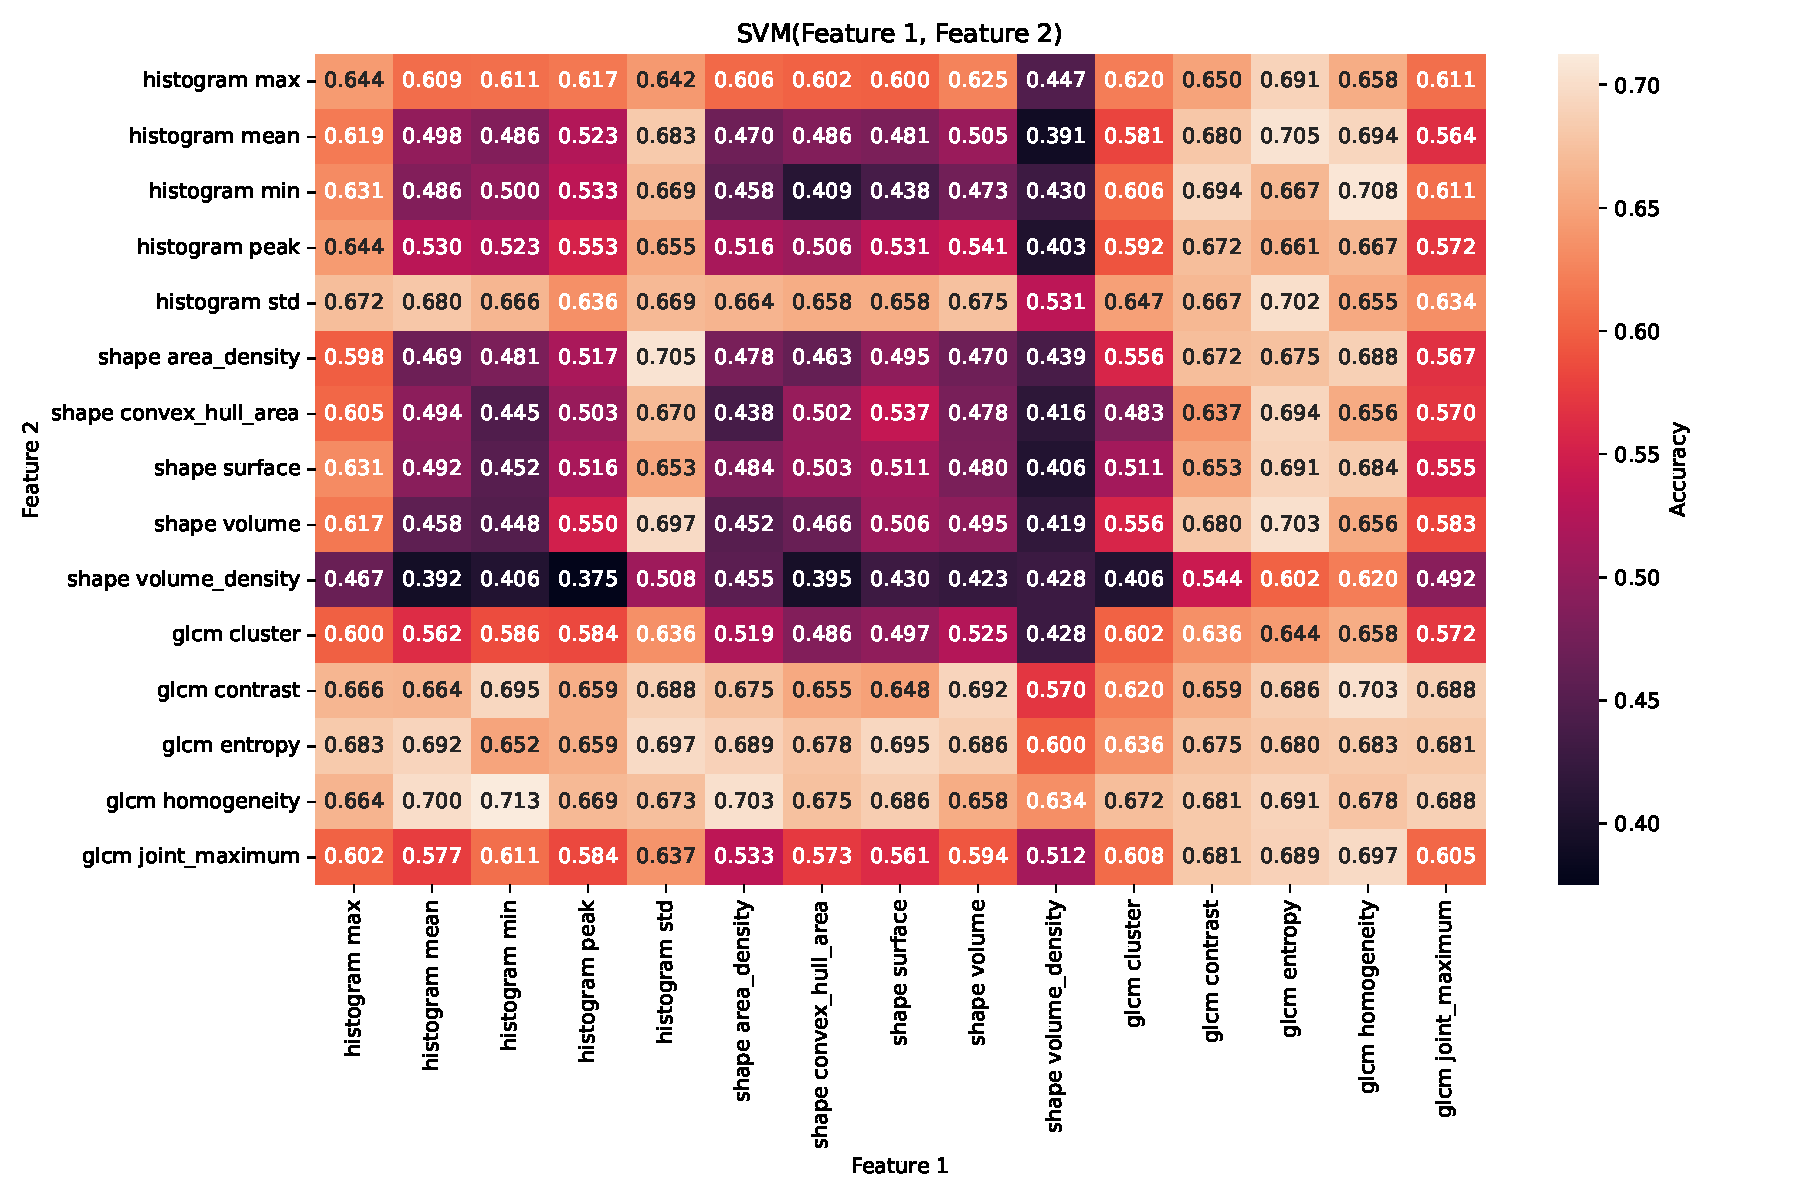
\includegraphics[width=1.2\textwidth]{Figures/feature_pairs4}}
\caption{Heatmap of the accuracy obtained by the SVM model training on different feature pairs. The SVM accuracies are the average 
of $20$ cross-validation cycles training and predicting test data of relative size $0.25$.
The slack constant and GRBF kernel factor are set to $C=10^4$  $\gamma=1 $ respectively. }
\label{fig:Figures-feature_pairs4}
\end{figure}

\begin{figure}[H]
\centering
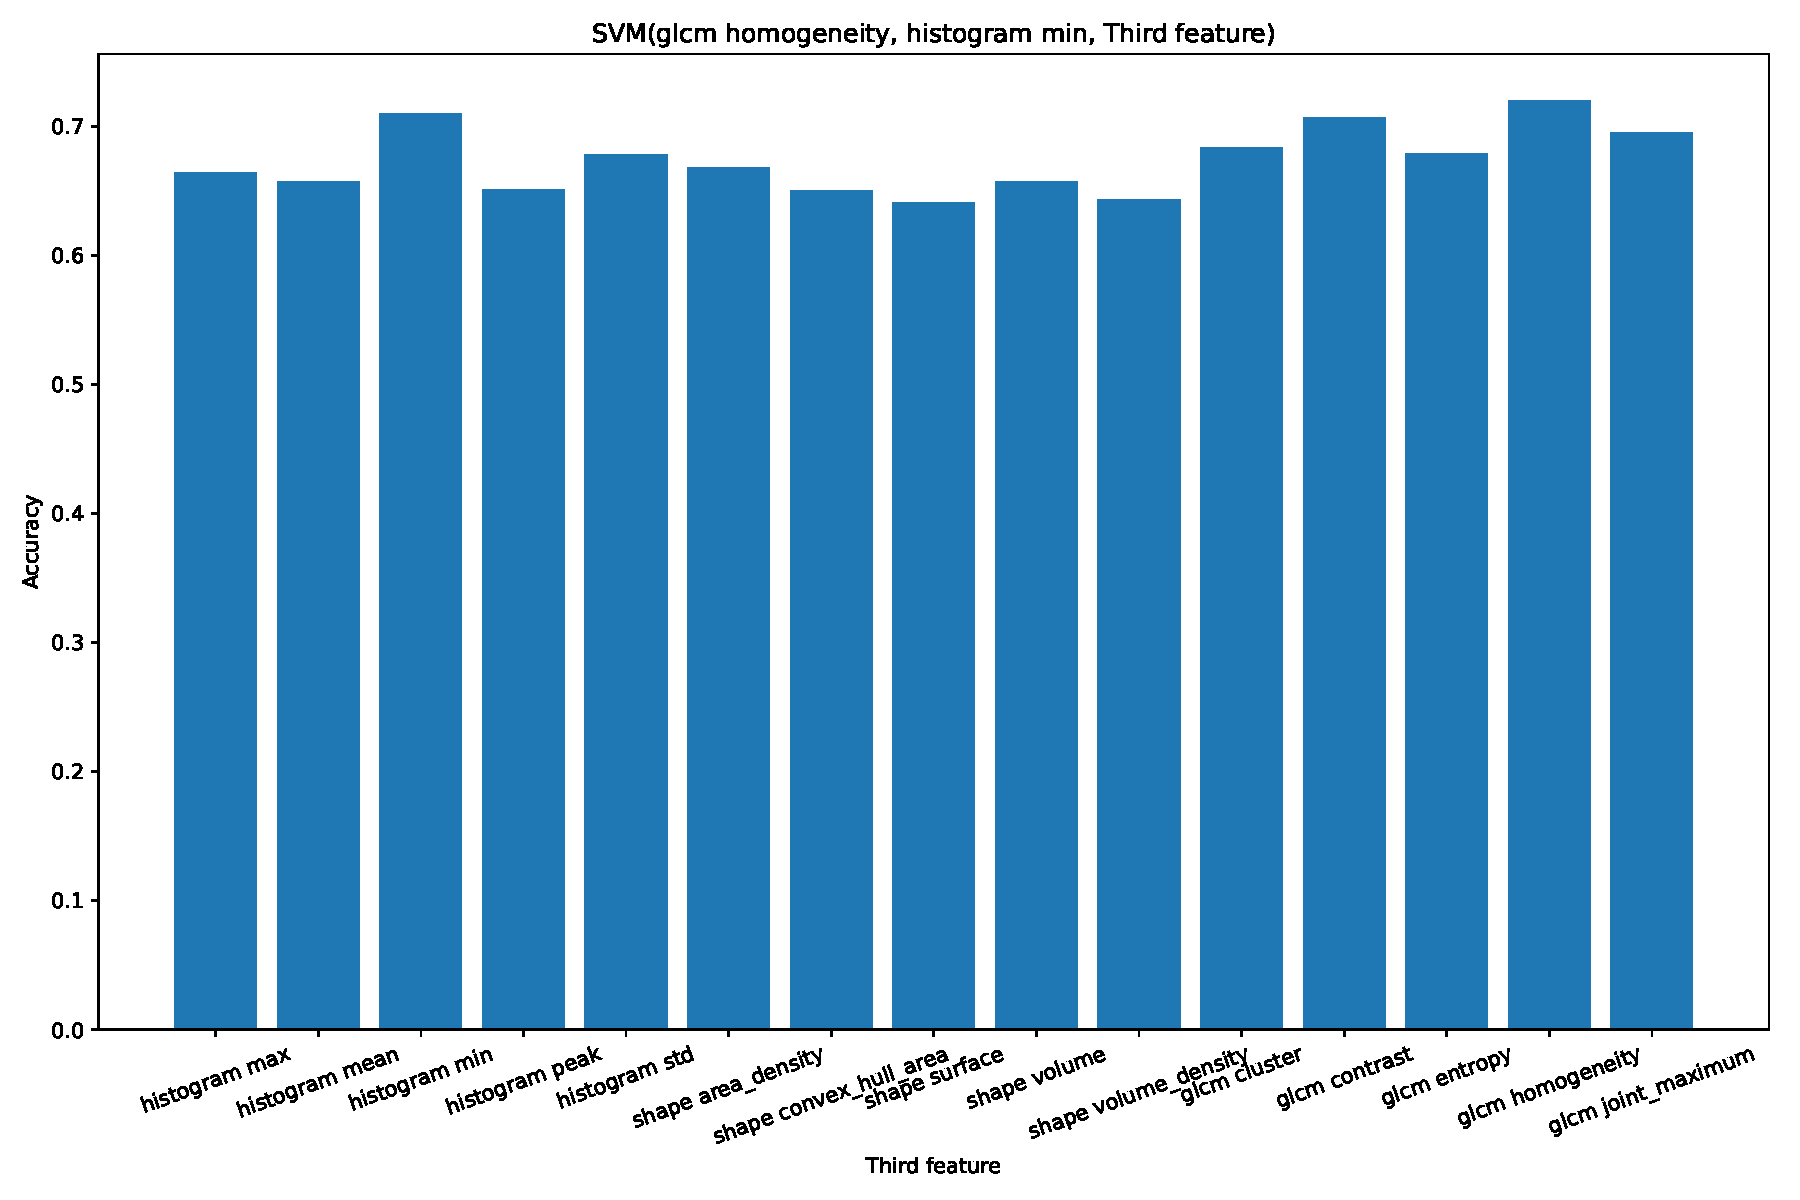
\includegraphics[width=1\textwidth]{Figures/third_feature4}
\caption{Bar plot of the accuracy obtained adding a third feature in the data used 
by the SVM model. The accuracies are the average 
of $50$ cross-validation cycles training and predicting test data of relative size $0.25$.
The slack constant and GRBF kernel factor are set to $C=10^4$  $\gamma=1 $ respectively. }
\label{fig:Figures-third_feature4}
\end{figure}



